\section{Implementation platforms}
%\label{sec:implementation platforms}

A platform refers to the combination of hardware resources (computation, communication, and memory) and the software (tasks, messages, mapping and scheduling) required to deploy an algorithm/application on the hardware effectively.
The execution time of tasks - sensing and processing (\taskS), control compute (\taskC), and actuation (\taskA) - of an \gls{ibc} system is dependent on the platform configuration.
The relatively straightforward way to reduce the long sensing delay is to have a processor with a high clock speed. 
However, this increases the cost of the processor. Moreover, the scaling of clock speed has reached its limits because of physical constraints in chip manufacturing and operation.
Another option to cope with long sensing delay is to have a platform with multiprocessor capabilities that enable concurrent parallel and pipelined execution of tasks.
A multiprocessor platform is economical due to the impact of Moore's law and is common nowadays.

In this thesis, two kinds of multiprocessor platforms are considered for the \gls{ibc} system implementation.
First, a \gls{compsoc} platform~\cite{hansson2009compsoc} is considered.
The \gls{compsoc} platform offers a composable and (timing) predictable implementation for the designer. 
The results of this thesis can be effectively applied to such predictable platforms without any adaptation.
Second, state-of-the-art industrial platforms are considered.
Predictability and composability are usually not offered in an industrial platform. 
We adapt our design approach for the industrial platforms NVIDIA Drive PX2 and NVIDIA AGX Xavier~\cite{nvidiaAGX} to demonstrate its applicability in an industrial context.
Our design approach is also applicable for more recent industrial platforms like the Tesla \gls{fsd} computer~\cite{talpes2020compute} and NVIDIA Drive AGX~\cite{nvidiadrive}.

\begin{figure}[t]
\centerline{
    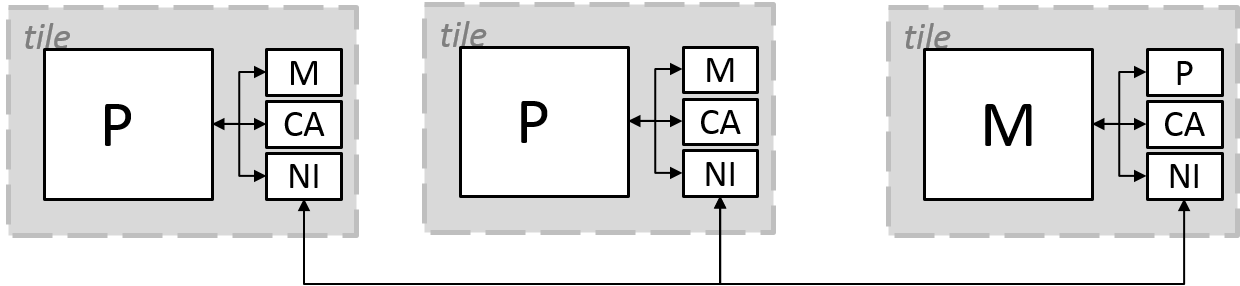
\includegraphics[width=0.8\textwidth]{01_intro/images/mpsoc_wo_index.png}
    }
    \caption{A \gls{compsoc} platform with two processor tiles and a memory tile connected through a \gls{noc}.}
    \label{fig:mpsoc}
    %\vspace{-2em}
\end{figure}

\subsection{\Gls{compsoc}}
\label{sec:compsoc}
\gls{compsoc} offers a tile-based architecture~\cite{stuijk2007} (see Fig.~\ref{fig:mpsoc}). Each tile has a processor $P$, memory $M$, communication assist $CA$ and network interface $NI$. 
Each processor tile has a microblaze processor, the memory tile contains an external memory interface, e.g., \gls{dram}, and the \gls{noc} provides interconnection between the tiles.
The platform is predictable with tight bounds on \glspl{wcet} of tasks and composable so that applications sharing the platform do not interfere with each other. 
A scheduler performs (re)configuration and time-triggered task execution. 

\begin{figure}[ht]
\centerline{
    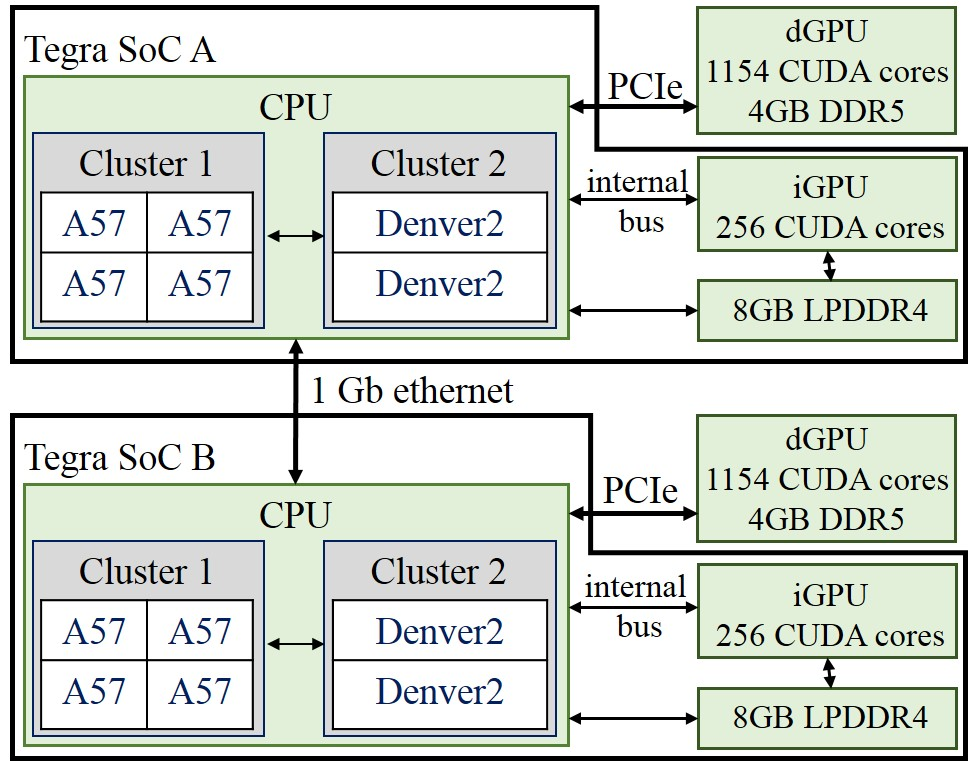
\includegraphics[width=0.65\textwidth]{01_intro/images/drive_platform.jpg}
    }
    \caption{NVIDIA Drive PX2 platform structure. LPDDR4 and DDR5 are the memory blocks. Each CPU cluster also has internal instruction and data memory (not shown in the graph).}
    \label{fig:drive_platform}
    %\vspace{-2em}
\end{figure}
\subsection{NVIDIA Drive PX2}
\label{sec:nvidia_px2}
The NVIDIA Drive PX2~\cite{nvidiadrive} platform consists of two Tegra \glspl{soc} that communicate to each other via ethernet. Each Tegra \gls{soc} has two \gls{cpu} clusters (see Fig.~\ref{fig:drive_platform}). One
cluster contains four ARM Cortex A57 cores and the other
contains two NVIDIA Denver2 cores. The clusters are connected
through a high-performance network interconnect. Each of the
Tegra \glspl{soc} also has two \glspl{gpu} -
an \gls{igpu} and a \gls{dgpu} with maximum clock rates of 1.27 and 1.29 GHz respectively. The \gls{igpu} has 256 CUDA cores and the \gls{dgpu} has 1154 CUDA cores. The \glspl{gpu} are accessed via the respective \glspl{cpu} in the \gls{soc}. The Ubuntu 16.04 LTS \gls{os} runs on the \gls{cpu} platform. 

\subsection{NVIDIA AGX Xavier}
\label{sec:nvidia_agx}
The NVIDIA AGX Xavier platform (illustrated in Fig.~\ref{fig:nvidia_platform}) consists of a Xavier \gls{soc} and other components explained in~\cite{nvidiaAGX}.
The \gls{cpu} complex consists of four heterogeneous dual-core NVIDIA Carmel \gls{cpu} clusters based on ARMv8.2 with a maximum clock frequency of 2.26GHz. 
The \gls{gpu} with a maximum clock frequency of 1.37GHz is accessed via the \glspl{cpu} in the \gls{soc}. The Ubuntu 18.04 LTS \gls{os} runs on the \gls{cpu} platform.
\begin{figure}[t]
\centerline{
    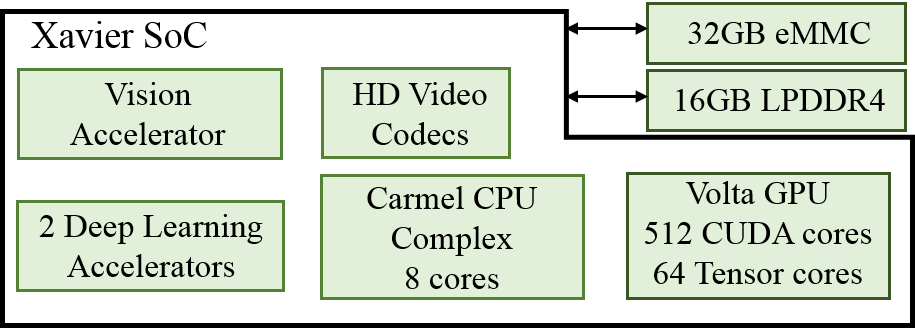
\includegraphics[width=0.65\textwidth]{01_intro/images/platform.png}
    }
    \caption{NVIDIA AGX Xavier platform block diagram. LPDDR4 and eMMC are the memory blocks. Each \gls{cpu} cluster also has internal instruction and data memory (not shown in the graph).}
    \label{fig:nvidia_platform}
    %\vspace{-2em}
\end{figure}